% Options for packages loaded elsewhere
\PassOptionsToPackage{unicode}{hyperref}
\PassOptionsToPackage{hyphens}{url}
%
\documentclass[
]{article}
\usepackage{amsmath,amssymb}
\usepackage{lmodern}
\usepackage{ifxetex,ifluatex}
\ifnum 0\ifxetex 1\fi\ifluatex 1\fi=0 % if pdftex
  \usepackage[T1]{fontenc}
  \usepackage[utf8]{inputenc}
  \usepackage{textcomp} % provide euro and other symbols
\else % if luatex or xetex
  \usepackage{unicode-math}
  \defaultfontfeatures{Scale=MatchLowercase}
  \defaultfontfeatures[\rmfamily]{Ligatures=TeX,Scale=1}
\fi
% Use upquote if available, for straight quotes in verbatim environments
\IfFileExists{upquote.sty}{\usepackage{upquote}}{}
\IfFileExists{microtype.sty}{% use microtype if available
  \usepackage[]{microtype}
  \UseMicrotypeSet[protrusion]{basicmath} % disable protrusion for tt fonts
}{}
\makeatletter
\@ifundefined{KOMAClassName}{% if non-KOMA class
  \IfFileExists{parskip.sty}{%
    \usepackage{parskip}
  }{% else
    \setlength{\parindent}{0pt}
    \setlength{\parskip}{6pt plus 2pt minus 1pt}}
}{% if KOMA class
  \KOMAoptions{parskip=half}}
\makeatother
\usepackage{xcolor}
\IfFileExists{xurl.sty}{\usepackage{xurl}}{} % add URL line breaks if available
\IfFileExists{bookmark.sty}{\usepackage{bookmark}}{\usepackage{hyperref}}
\hypersetup{
  pdftitle={Regression Analysis of Apartment Building Evaluation in Toronto},
  pdfauthor={Alexandre Haulard},
  hidelinks,
  pdfcreator={LaTeX via pandoc}}
\urlstyle{same} % disable monospaced font for URLs
\usepackage[margin=1in]{geometry}
\usepackage{graphicx}
\makeatletter
\def\maxwidth{\ifdim\Gin@nat@width>\linewidth\linewidth\else\Gin@nat@width\fi}
\def\maxheight{\ifdim\Gin@nat@height>\textheight\textheight\else\Gin@nat@height\fi}
\makeatother
% Scale images if necessary, so that they will not overflow the page
% margins by default, and it is still possible to overwrite the defaults
% using explicit options in \includegraphics[width, height, ...]{}
\setkeys{Gin}{width=\maxwidth,height=\maxheight,keepaspectratio}
% Set default figure placement to htbp
\makeatletter
\def\fps@figure{htbp}
\makeatother
\setlength{\emergencystretch}{3em} % prevent overfull lines
\providecommand{\tightlist}{%
  \setlength{\itemsep}{0pt}\setlength{\parskip}{0pt}}
\setcounter{secnumdepth}{-\maxdimen} % remove section numbering
\usepackage{booktabs}
\usepackage{siunitx}
\newcolumntype{d}{S[input-symbols = ()]}
\usepackage{longtable}
\usepackage{array}
\usepackage{multirow}
\usepackage{wrapfig}
\usepackage{float}
\usepackage{colortbl}
\usepackage{pdflscape}
\usepackage{tabu}
\usepackage{threeparttable}
\usepackage{threeparttablex}
\usepackage[normalem]{ulem}
\usepackage{makecell}
\usepackage{xcolor}
\ifluatex
  \usepackage{selnolig}  % disable illegal ligatures
\fi

\title{Regression Analysis of Apartment Building Evaluation in Toronto}
\author{Alexandre Haulard}
\date{Assignment 2: STA304 - 20/10/2021}

\begin{document}
\maketitle

~ ~ ~

\hypertarget{introduction}{%
\section{Introduction}\label{introduction}}

\hypertarget{analysis-goal}{%
\subsection{Analysis Goal}\label{analysis-goal}}

The goal of this analysis is to use multiple linear regression models in
order to predict the evaluation score of a building. This prediction
will be based on three independent variables: the number of units in a
building, the age of the building, and the property type of the
building. This analysis is conducted using the Apartment Building
Evaluation data set provided by the Toronto open data portal (\emph{1.
``Open Data''}). The analysis is performed using buildings that have
been built in the last 40 years (i.e., after 1980), and evaluated in
2020. The reason is that a great proportion of buildings have been built
during the 1950-1970's baby boom and are concentrated in specific wards
of Toronto.

This analysis is relevant to Torontonians who are owner of an apartment
building property or seeking to buy or rent a property in Toronto.
Additionally, the analysis is relevant to people seeking social housing
in Toronto. This is because the data provides information about private
properties, Toronto Community Housing, but also social housing.

The apartment building evaluation program is called ``RentSafeTO''. It
was implemented in 2017 by the city of Toronto in order to protect
Torontonians by making sure they are provided with information to live
in the best conditions possible. During evaluations, Bylaw Enforcement
Officers inspect common areas, mechanical and security systems, parking
and exterior grounds (\emph{2. ``City of Toronto''}). Buildings are then
provided with a percentage score. A higher score implies a building
respects safety regulations and is well maintained.

Now having introduced the importance of the ``RentSafeTO'' program which
aims to improve the well being of Torontonians, we can formulate a
research question for our analysis: \emph{\textbf{Can the evaluation
score of a building be predicted such that there exists a linear
relationship where the evaluation score is dependent on the number of
units, property type, and age of the building?}}

\hypertarget{terminology}{%
\subsection{Terminology}\label{terminology}}

In order to understand the following analysis, let's define the terms
that will be used extensively.

\begin{itemize}
\item
  \textbf{Private Property}: These are buildings operated by private
  owners and/or investment firms. They are run in a for-profit manner.
\item
  \textbf{TCHC}: The acronym stands for Toronto Community Housing. It is
  a social housing provider in Canada wholly owned by the City of
  Toronto that operates in a non-profit manner. TCHC has 2,100 buildings
  and 50 million square feet of residential space, which represent a \$9
  billion public asset (\emph{3. ``TCHC, Who We Are .''}).
\item
  \textbf{Social Housing}: This represents all other Toronto social
  housing providers that are not TCHC.
\end{itemize}

\hypertarget{hypothesis}{%
\subsection{Hypothesis}\label{hypothesis}}

Before exploring the data and computing the regression model, let's
formulate three hypotheses for potential results.

\begin{enumerate}
\def\labelenumi{\arabic{enumi}.}
\item
  Intuitively, buildings with a younger age should be easier to maintain
  than older ones. Therefore, we expect younger buildings to have a
  higher evaluation score.
\item
  Supposing that buildings with higher evaluation scores are more in
  demand, we would expect their value to increase. Therefore, it is
  expected that properties of type private have a higher evaluation
  score. My reasoning behind this is that private property owners have
  incentives to see their assets go up in value which happens when
  demand for an asset is high.
\item
  Finally, I hypothesize that the direction of the relationship between
  evaluation score and the number of units in a building is positive.
  Intuitively, buildings with more units would be harder to maintain
  which would negatively affect the evaluation score. On the other hand,
  the maintenance cost should be less challenging to handle for
  buildings with more units. This is because the cost of maintaining
  common areas can be divided among more people such that maintenance
  fees per unit are lower. This would positively affect the
  relationship. I hypothesize that the latter economic reason has a
  stronger effect; thus, the relationship would be positive.
\end{enumerate}

The purpose of the following section is to showcase the data to get a
better understanding of what we are working with.

\hypertarget{data}{%
\section{Data}\label{data}}

\hypertarget{collection-process}{%
\subsection{Collection Process}\label{collection-process}}

The data that will be used for this analysis are published on the
Toronto Open Data Portal by the Toronto Municipal Licensing \& Standards
(\emph{1. ``Open Data''}). The data is refreshed daily. For this
analysis, the data was downloaded locally on October 20, 2021.
Therefore, no entry added after this date will be captured by our
analysis. The data provides an entry for each year a building was
evaluated. These entries contain the overall score evaluation (as a
percentage), geographic information (Ward, Latitude, Longitude,
Address), the property type, number of units and storeys, but also
detailed score evaluation (out of five) about specific areas evaluated
(Entrance Lobby, Stairwell, Elevator, Security, Parking Area\ldots). The
formula to calculate the overall score is as follows: sum of all
assigned detailed scores during the evaluation \(\div\) (number of
unique items reviewed \(\times\) 5).

\hypertarget{cleaning-process}{%
\subsection{Cleaning Process}\label{cleaning-process}}

In the original data, each entry corresponds to a building evaluation
made in a certain year. A building could appear more than once in the
data if it was evaluated in different years. For this analysis, we only
use buildings that were evaluated in 2020. Thus, we remove all
observations which do not have an evaluation year of 2020. In the
cleaned data frame, a building will not appear twice, as it can only be
evaluated once a year.

As mentioned in the introduction, we are only interested in buildings
built in 1980 or after. All other observations for buildings built
before 1980 are removed. Additionally, observations where the number of
units is below 248 are removed. This is because, among each property
type, Social Housing has the lowest max at 248. The rational for doing
this is that we want to make sure our linear regression model is
comparable given a property type.

The original data contains a variable Year Built. This variable is
removed, but used to create a new variable named Age where Year Built is
subtracted from 2021. For example, a given observation in the cleaned
data frame will not display the variable Year Built being 1980, but
instead will display the variable Age being 31.

Finally, we are only interested in the overall score, the property type,
the age, and the number of units in a given building. Thus, we can
remove all other variables and are left with four variables in the
cleaned data frame.

\hypertarget{definition-of-the-variables-that-will-be-used-extensively}{%
\subsection{Definition of the variables that will be used
extensively}\label{definition-of-the-variables-that-will-be-used-extensively}}

This subsection serves as reference for the definition of the variables
that are used throughout the analysis.

\begin{itemize}
\item
  \textbf{Age}: This variable describes how old a building is. If a
  building was built in 2005, its age will be 16.
\item
  \textbf{Score}: This variable describes the evaluation percentage
  score for a given building that was evaluated in 2020. A low score
  implies that a building is poorly maintained.
\item
  \textbf{Type}: This variable describes the property type of a
  building. There are three possible values for this variable: Private,
  TCHC, and Social Housing. These were defined previously in the
  terminology section.
\item
  \textbf{Number of Units}: This variable provides the number of units
  in a given building.
\end{itemize}

\hypertarget{numerical-summary-statistics}{%
\subsection{Numerical Summary
Statistics}\label{numerical-summary-statistics}}

Firstly, let's consider that there are 103 observations in our cleaned
data frame. Additionally, we have one categorical variable named Type.
This variable contains 23 observations for Private properties, 26 for
TCHC properties, and 54 for other Social Housing properties. Let's
compute a numerical summary for each continuous variable we have.

\begin{table}[!htbp] \centering 
  \caption{Numerical Summaries of Continuous Variables} 
  \label{} 
\begin{tabular}{@{\extracolsep{5pt}}lccccccc} 
\\[-1.8ex]\hline 
\hline \\[-1.8ex] 
Statistic & \multicolumn{1}{c}{Mean} & \multicolumn{1}{c}{St. Dev.} & \multicolumn{1}{c}{Min} & \multicolumn{1}{c}{Pctl(25)} & \multicolumn{1}{c}{Median} & \multicolumn{1}{c}{Pctl(75)} & \multicolumn{1}{c}{Max} \\ 
\hline \\[-1.8ex] 
Age & 26.427 & 11.365 & 2 & 18 & 29 & 36 & 41 \\ 
Score & 81.301 & 8.870 & 61 & 75 & 81 & 87.5 & 100 \\ 
Number of Units & 92.544 & 69.017 & 10 & 28.5 & 83 & 152.5 & 248 \\ 
\hline \\[-1.8ex] 
\end{tabular} 
\end{table}

The first variable summary statistic provided by Table 1 is Age. It has
a mean of 26.427 which differs from the median of 29. This can be
interpreted in the following way: most of the building in our data were
built in the 1990's. Age has a minimum of 2 which means that the last
property built was in 2019.

The summary statistic also provides a better idea of the evaluation
score system. It has a mean of 81.301 and a standard deviation of 8.87.
In this context, the standard deviation is quite low so the buildings
would be compared by very few percentage points when using the
evaluation score.

The minimum number of units is 10. This makes sense because the
``RentSafeTO'' program only evaluates buildings with 10 units or more.

The Number of Units has a mean of 92.544 and a remarkably high standard
deviation of 69. For this reason, let's compute the means of each
continuous variable conditional on the property type to see if they
differ greatly.

~

\begin{table}[ht]
\centering
\caption{Mean Summary by Property Type} 
\begin{tabular}{lrrr}
  \hline
Type / Mean & Age & Score & Number of Units \\ 
  \hline
Private & 18.70 & 86.30 & 84.04 \\ 
  Social Housing & 27.91 & 80.17 & 78.30 \\ 
  TCHC & 30.19 & 79.23 & 129.65 \\ 
   \hline
\end{tabular}
\end{table}

~

First, notice that Private properties are on average younger than both
TCHC properties and other Social Housing organizations.

Secondly, the mean evaluation score of private properties stands at
86.304. It is way above the mean evaluation score of both TCHC
properties, and other Social Housing. This is in line with hypothesis 2.

Finally, the mean for Private and Social Housing properties are quite
close standing at 84.043 and 78.296. These two values are quite far from
the mean number of units for TCHC properties which stands at 129.654.
This explains the high standard deviation founded in Table 1 for the
number of units not conditional on the property type.

\hypertarget{visualizing-the-data}{%
\subsection{Visualizing the Data}\label{visualizing-the-data}}

Let's use three scatter plots for each of the property types mapping
Evaluation Score dependent on the number of units in a building. A
continuous scale representing Age is added.

~

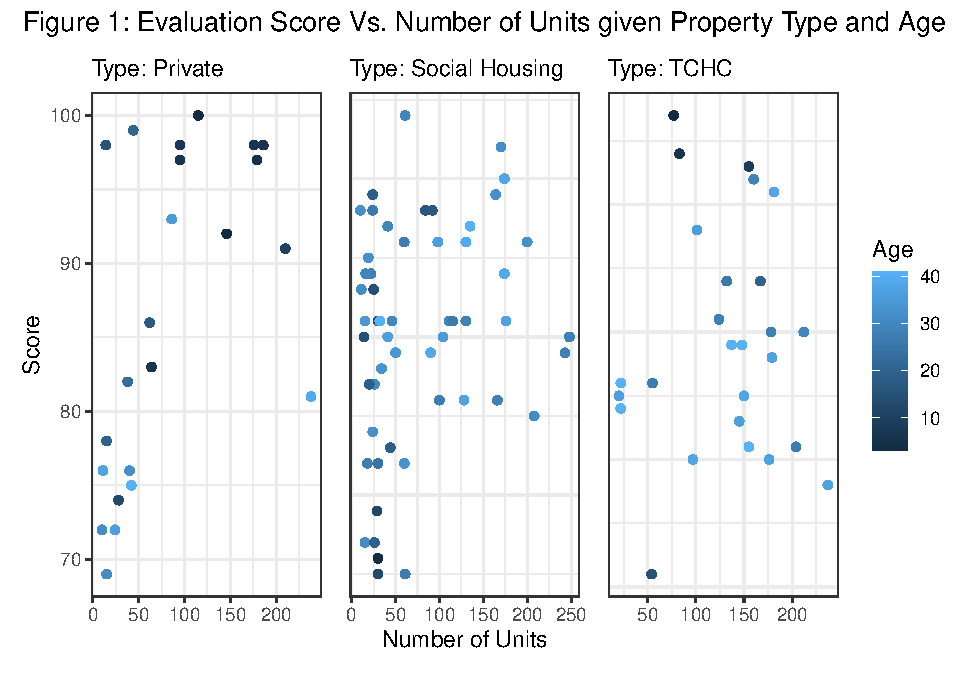
\includegraphics{A2_files/figure-latex/unnamed-chunk-5-1.pdf}

Figure 1 contains a lot of information but is nevertheless easy to
understand. Each of the three scatter plots represent observations for
each of the three property types: Private, Social Housing, and TCHC. The
dependent variable on the y-axis is the evaluation score of a building.
The independent variable on the x-axis is the number of units in a
building. The continuous scale represents the age of buildings. A darker
blue means a building is younger while a lighter blue means a building
is older.

A multiple linear regression model is appropriate to predict the
evaluation score as we took care of the issue regarding outliers in the
data section. A multiple linear regression of the dependent variable
Score on the following independent variables number of units, Age, and
Property Type will be performed. The number of units should be
considered as our main independent variable of interest while the two
other independent variables age and type should be considered as control
variables. This will be defined more precisely in the next section
called `Methods' where the multiple linear regression model is
introduced.

\hypertarget{methods}{%
\section{Methods}\label{methods}}

The aim of this section is to introduce multiple linear regression,
assumptions, and selection techniques to compare models.

\hypertarget{multiple-linear-regression-models}{%
\subsection{Multiple Linear Regression
Models}\label{multiple-linear-regression-models}}

Multiple linear regression generalizes the simple linear regression
model by allowing for many terms in a mean function rather than just one
intercept and one slope (\emph{4. Weisberg, Sanford}).

The simple linear regression model is defined as follows:
\(y=\beta_0 + \beta_1x + \epsilon\). The goal of the simple linear
regression model was to estimate the \(\beta_0\) and \(\beta_1\)
parameters to obtain a function that predicts the independent variable
\(y\) given any \(x\). The Greek letter \(\epsilon\) is called the error
term. It will not be rigorously defined here, but the intuition behind
\(\epsilon\) is that it captures the inaccuracy in the model. It
explains the difference between the theoretical value of the model and
the actual observed results (\emph{5. Holmes, Alexander, et al.}).

The multiple linear regression model is simply an expansion of the
simple linear regression model where we can add as many
\(x_1, x_2, ..., x_k\) as we wish. It follows that for each \(x_i\)
added predictor, we need to estimate an additional \(\beta_i\). The
estimate of the \(\beta\) parameters is found using ordinary
least-squares. Here is a reference for the reader interested in the
mathematics of OLS (\emph{4. Weisberg, Sanford}). For our analysis, the
estimation of the parameters will be handled by the R statistical
programming software. The multiple linear regression model is as
follows:

\[y=\beta_0 + \beta_1x_1 + \beta_2x_2 + ... + \beta_kx_k + \epsilon\]

The main idea behind adding \(x_2,..., x_k\) is to explain the part of
\(y\) that has not already been explained by \(x_1\). Now, to relate
this theory to our original problem, we will introduce four linear
regression models. First, a simple linear regression of Score on Number
of Units. Then for the second model, we add a second independent
variable Age to create a multiple linear regression model. The third
model is an extension of the second where we add the independent
variable Type.

\begin{itemize}
\tightlist
\item
  \textbf{Model 1}:
  \(Score_i = \beta_0 + \beta_1NumUnits_i + \epsilon_i\)
\end{itemize}

The interpretation of this model is simple: if the number of units
increases by one, then the score would increase by \(\beta_1\).

\begin{itemize}
\tightlist
\item
  \textbf{Model 2}:
  \(Score_i = \beta_0 + \beta_1NumUnits_i + \beta_2Age_i + \epsilon_i\)
\end{itemize}

The variable Type we will add to the third model is categorical. This
means we need to add two binary variables for the three categories.

\begin{itemize}
\tightlist
\item
  \textbf{Model 3}:
  \(Score_i = \beta_0 + \beta_1NumUnits_i + \beta_2Age_i + \beta_3(Type = SH) + \beta_4(Type=TCHC) + \epsilon_i\)
\end{itemize}

In the case of an observation where the Type is Social Housing, we set
\(SH= 1\) and \(TCHC=0\). If Type were to be Private, we set \(SH= 0\)
and \(TCHC=0\).

\begin{itemize}
\tightlist
\item
  \textbf{Model 4}:
  \(Score_i = \beta_0 + \beta_1NumUnits_i + \beta_2Age_i + \beta_3(Type = SH) + \beta_4(Type=TCHC) + \beta_5(Type = SH)\cdot Age_i + \beta_6(Type=TCHC) \cdot Age_i +\epsilon_i\)
\end{itemize}

In this model, we have introduced an interaction effect by multiplying
the type variable by the age variable. If dependence between these
variables exists, model 4 should provide more accurate responses than
model 3.

\hypertarget{assumptions}{%
\subsection{Assumptions}\label{assumptions}}

Readers not interested in the specifics of linear regression may skip
this section. Before introducing selection techniques, let's introduce a
few assumptions about the linear regression models:

\begin{enumerate}
\def\labelenumi{\arabic{enumi}.}
\item
  \emph{The model is linear in parameters.} This assumption is met for
  all four models.
\item
  \emph{Random Sampling, i.e., \((x_{1i},…,x_{ki},y_i)\), \(i =1,…,n\)
  are i.i.d.} This assumption is met as we have used all the existing
  observations in our setting.
\item
  \emph{No Perfect Collinearity.} This assumption is met for all four
  models as our variables do not constitute any linear combination of
  each other, and do not sum to a constant.
\item
  \emph{\(E(\epsilon| x_1,…, x_k) = 0\).} We will check if this
  assumption is met in the `Results' section.
\end{enumerate}

All these assumptions were retrieved from the Wooldridge's textbook
referenced in the Bibliography section (\emph{6. Wooldridge, Jeffrey
M.}).

\hypertarget{model-selection-techniques}{%
\subsection{Model Selection
Techniques}\label{model-selection-techniques}}

There are three techniques that will be used to determine which of the
four models is the most appropriate.

\begin{itemize}
\item
  \textbf{F-Test}: This is an hypothesis test which is formulated as
  follows; \(H_0: \beta_1,...,\beta_k =0\). This says that none of the
  predictors are linearly related to the response. If we can reject the
  null hypothesis, then at least one predictor is linearly related to
  the response. We will perform this test on each model, and reject the
  null hypothesis if we find a p-value below 0.05 (\emph{7.
  ``STA302/1001''}). In other words, if a model has a p-value greater
  than 0.05, it will not be considered.
\item
  \textbf{AIC}: The equation of this test is as follows;
  \(AIC = 2k-2ln(\hat{L})\). The number of predictors is \(k\), so more
  predictors increases the value of AIC. \(\hat{L}\) is the maximum
  value of the likelihood function. Therefore, if our model fits well,
  the second term of AIC would be higher. This means AIC would be lower.
  Thus, when comparing models, we are looking for the one with the
  lowest AIC (\emph{8. ``Akaike Information Criterion.''}).
\item
  \(\mathbf{R_{adj}^2}\): This test is called the adjusted coefficient
  of determination. A higher value is better when comparing it between
  models. It is used to measure the proportion of the variation in the
  dependent variable that is predictable from the independent variables
  (\emph{9. ``Coefficient of Determination.''}). As opposed to \(R^2\),
  \(R_{adj}^2\) takes into account the size of the model. This means
  adding predictors brings down \(R_{adj}^2\), but if the model fits
  better with the added predictors, \(R_{adj}^2\) goes up.
\end{itemize}

The computation of all these test statistics will be handled by R. Let's
finally compute the results of all the methodologies introduced.

\hypertarget{results}{%
\section{Results}\label{results}}

\hypertarget{numerical-results}{%
\subsection{Numerical Results}\label{numerical-results}}

The next table outputs the results of the estimations of parameters
(along with their standard errors in parenthesis) for each model, and
the test statistics to compare them.

\begin{table}[!h]

\caption{\label{tab:unnamed-chunk-7}Estimation of Parameters for Linear Regression Models}
\centering
\begin{tabular}[t]{lcccc}
\toprule
  & Model 1 & Model 2 & Model 3 & Model 4\\
\midrule
(Intercept) & \num{78.760} & \num{86.126} & \num{87.464} & \num{93.887}\\
 & (\num{1.440}) & (\num{2.212}) & (\num{2.349}) & (\num{2.966})\\
Number of Units & \num{0.027} & \num{0.032} & \num{0.037} & \num{0.021}\\
 & (\num{0.012}) & (\num{0.012}) & (\num{0.012}) & (\num{0.012})\\
Age &  & \num{-0.295} & \num{-0.230} & \num{-0.502}\\
 &  & (\num{0.071}) & (\num{0.074}) & (\num{0.115})\\
Type: Social Housing &  &  & \num{-3.808} & \num{-21.443}\\
 &  &  & (\num{2.087}) & (\num{4.475})\\
Type: TCHC &  &  & \num{-6.134} & \num{-5.040}\\
 &  &  & (\num{2.471}) & (\num{4.864})\\
Age × Type: Social Housing &  &  &  & \num{0.719}\\
 &  &  &  & (\num{0.171})\\
Age × Type: TCHC &  &  &  & \num{0.091}\\
 &  &  &  & (\num{0.173})\\
\midrule
N & \num{103} & \num{103} & \num{103} & \num{103}\\
F & \num{4.830} & \num{11.533} & \num{7.582} & \num{9.489}\\
p & \num{0.03025481} & \num{3.113e-05} & \num{2.303e-05} & \num{4e-08}\\
AIC & \num{742.1} & \num{727.6} & \num{725.2} & \num{709.0}\\
AdjustedR-Squared & \num{0.036} & \num{0.171} & \num{0.205} & \num{0.333}\\
\bottomrule
\end{tabular}
\end{table}

~

\textbf{\emph{Interpretation of estimated parameters}}

The number of units parameter varies a little between the 4 models. It
is estimated at 0.027 in Model 1. As we add variables, it goes up to
0.032 and 0.037 in Model 2 and 3. Interestingly, it goes down to 0.021
in Model 4 after the interaction variable is added. The number of units
parameter in Model 4 can be interpreted in the following way: Holding
all other variables constant, increasing the number of units by 1 will
increase the apartment evaluation score by 0.021.

Model 2, 3, and 4 introduce a negative relationship between the Age of a
building and the evaluation score. This means that as a building gets
older, the evaluation score goes down.

Now, there is a nuance in Model 4 concerning the estimated parameter of
the interaction variable \(Age \times Type: Social Housing\). Its
estimate is 0.719 while the estimation of the parameter Age is -0.502.
Intuitively, this means that properties of type Social Housing have an
evaluation score that increases as they get older. The mathematical
reason for this is that we can factor the age variable in Model 4. Given
Type is Social housing we have
\(\beta_2Age_i + \beta_6Age_i \times(1) = (\beta_2 + \beta_6) Age_i\).
Plugging in the estimates we get \((-0.502 + 0.719)Age_i = 0.217Age_i\).
Thus, we can say that holding everything else constant and given a
property of type Social Housing, a 1 year increase in age will increase
the evaluation score by 0.217.

\textbf{\emph{Comparing Models Using the test statistics}}

The letter N is simply the number of observations we used to run our
models. The F-statistic for each model is shown in Table 3. Its only
relevance is to calculate the p-value. Every model has a p-value which
is less than 0.05. Therefore, we can reject the hypothesis that no
relationship exists between the response and at least one of the
variables. So far, all 4 models are valid so let's now check the AIC
statistic.

Recall that when comparing models, the one with the lower AIC is more
appropriate (given the models have been run on the same data set). Every
time we add a variable from Model 1 through Model 4, the AIC statistic
decreases. This means adding variables does not decrease the efficiency
of the models, and the models fit better and better. Consequently, Model
4 is the most appropriate according to the AIC statistic.

It was explained in the `Methods' section why a higher \(R_{adj}^2\) is
better. Model 4 has the highest \(R_{adj}^2\), so we can say it is the
most appropriate according to that test.

Finally, I conclude that Model 4 is the most appropriate since it is the
number one performer in the three previous tests.

\hypertarget{graphical-results}{%
\subsection{Graphical Results}\label{graphical-results}}

Let's graphically interpret the results of Model 4 by fitting regression
lines over the scatter plots from the Data section.

~

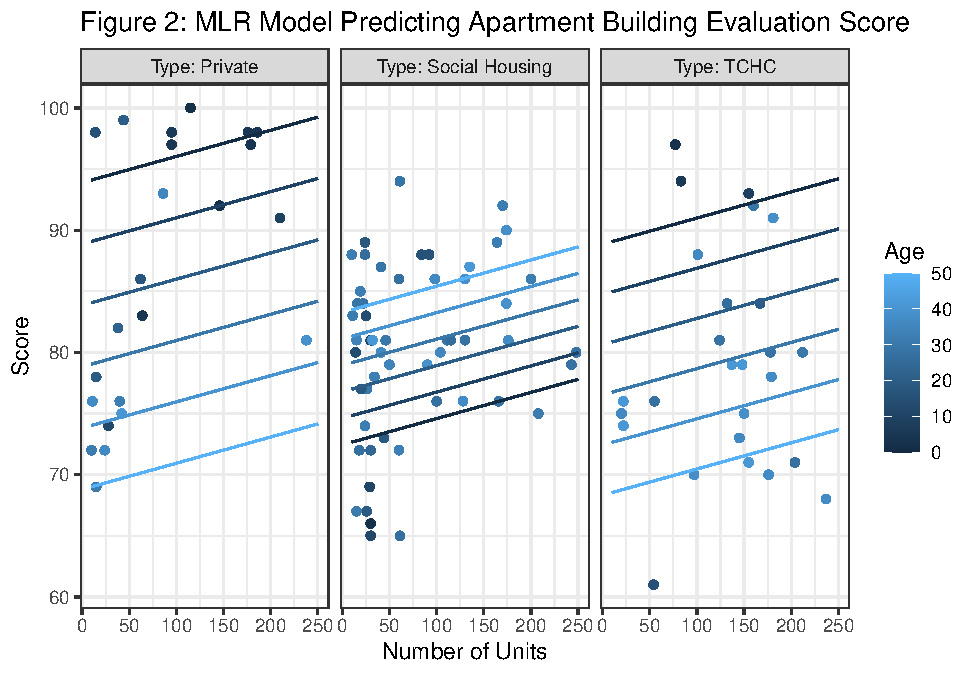
\includegraphics{A2_files/figure-latex/unnamed-chunk-8-1.pdf}

Given any property type, the relationship between number of units and
evaluation score is positive.

Looking at the Age continuous scale and understanding that each
regression line on one scatter plot represents a different age, we can
state that recently built Private properties are expected to have a
higher evaluation score than Social Housing and TCHC.

The nuance we previously stated is confirmed graphically. Light blue
(older) lines are higher than dark blue (younger) lines given a Social
Housing property type.

\hypertarget{testing-hypothesis-that-the-error-has-zero-conditional-means}{%
\subsection{Testing Hypothesis that the Error has Zero Conditional
Means}\label{testing-hypothesis-that-the-error-has-zero-conditional-means}}

Finally, I want to check graphically if hypothesis 4 holds,
i.e.~\emph{\(E(\epsilon| x_1,…, x_k) = 0\)}.

~

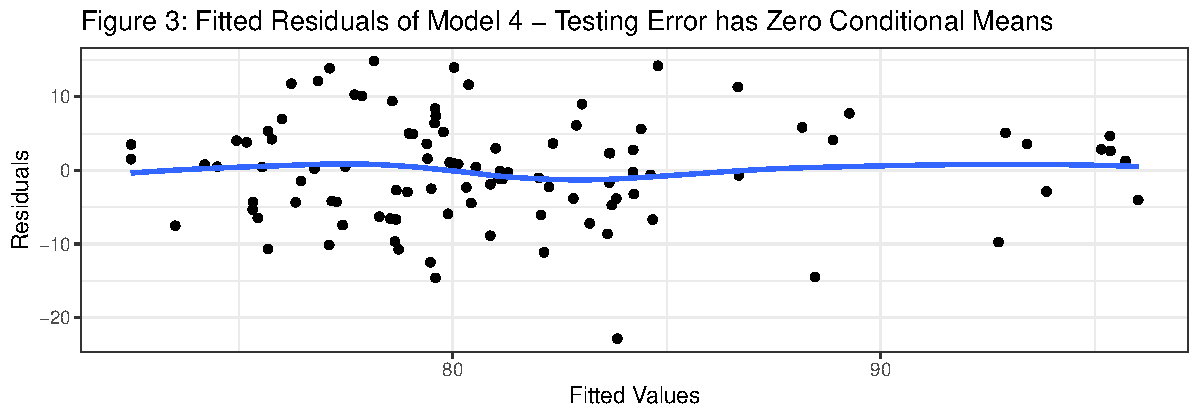
\includegraphics{A2_files/figure-latex/unnamed-chunk-9-1.pdf}

Assumption 4, \emph{\(E(\epsilon| x_1,…, x_k) = 0\)}, holds. Even though
the regression on residuals is not exactly a horizontal line equal to
zero, there is no concerning pattern and the divergence really is
negligible.

\hypertarget{conclusions}{%
\section{Conclusions}\label{conclusions}}

In this analysis, we have used a multiple linear regression model to
answer the following research question: \textbf{\emph{Can the evaluation
score of a building be predicted such that there exists a linear
relationship where the evaluation score is dependent on the number of
units, property type, and age of the building?}} The answer is yes. The
multiple linear regression model was valid as its assumptions were met,
and relevant relationships were found between evaluation score given the
number of units, property type, and the age of a building.

The first hypothesis stating that we expect younger buildings to have a
higher evaluation score is partially met. Results have shown that this
is true only for properties of type private and TCHC. Not for properties
of type Social housing.

The second hypothesis stating that it was expected properties of type
private have a higher evaluation score is true especially for recently
built buildings.

The last hypothesis stating that the direction of the relationship
between evaluation score and the number of units in a building is
positive is true for any observation. It does not depend on the property
type or age.

If there is one takeaway for this analysis, it is the last hypothesis
being true. The big picture is the following: It is economically easier
for apartments with many units to maintain common areas as the cost is
divided among each unit. Apartments with few units implies that the fees
paid per unit are high.

\hypertarget{weaknesses}{%
\subsection{Weaknesses}\label{weaknesses}}

The first obstacle faced in this analysis was that different apartment
types are built in bulk around the same time periods. This is what
happened during the baby boom from 1950 to 1970. Including these
buildings in our analysis would have made our model flawed.

\hypertarget{next-steps-and-discussion}{%
\subsection{Next Steps and Discussion}\label{next-steps-and-discussion}}

Some future work of relevance would be to reproduce this analysis on
buildings evaluated in 2021 once the year is done. This analysis about
buildings evaluated in 2020 would be compared to the future one. More
specifically, differences in the models and relationships would be
compared.

Another step to be taken is to analyze if Model 4 can be improved by
adding dependent variables to the model.

Finally, to summarize this report, we have shown using a multiple linear
regression model that there exists a positive relationship between a
building's evaluation score and the number of units in this building.

\newpage

\emph{All analysis for this report was programmed using
\texttt{R\ version\ 4.1.1}.}

\hypertarget{bibliography}{%
\section{Bibliography}\label{bibliography}}

\hypertarget{in-line-referencing}{%
\subsection{In Line Referencing}\label{in-line-referencing}}

\begin{enumerate}
\def\labelenumi{\arabic{enumi}.}
\item
  ``Open Data'' City of Toronto Open Data Portal,
  \url{https://open.toronto.ca/dataset/apartment-building-evaluation/.}
  (Last Accessed: October 20, 2021)
\item
  City of Toronto. ``Rentsafeto for Tenants.'' City of Toronto, 6
  Oct.~2021,
  \url{https://www.toronto.ca/community-people/housing-shelter/rental-housing-tenant-information/rental-housing-standards/apartment-building-standards/rentsafeto-for-tenants/.}
  (Last Accessed: October 20, 2021)
\item
  ``TCHC, Who We Are .'' About Us,
  \url{https://www.torontohousing.ca/who-we-are.} (Last Accessed:
  October 20, 2021)
\item
  WEISBERG, SANFORD. Applied Linear Regression. JOHN WILEY, 2021. (Last
  Accessed: October 20, 2021)
\item
  Holmes, Alexander, et al.~``The Regression Equation.'' Introductory
  Business Statistics, OpenStax, 31 Mar.~2015,
  \url{https://opentextbc.ca/introbusinessstatopenstax/chapter/the-regression-equation/.}
  (Last Accessed: October 20, 2021)
\item
  Wooldridge, Jeffrey M. Introductory Econometrics a Modern Approach.
  South-Western, Cengage Learning, 2020.
\item
  ``STA302/1001'' Methods of Data Analysis 1.
\item
  ``Akaike Information Criterion.'' Wikipedia, Wikimedia Foundation, 21
  Oct.~2021,
  \url{https://en.wikipedia.org/wiki/Akaike_information_criterion}.
\item
  ``Coefficient of Determination.'' Wikipedia, Wikimedia Foundation, 19
  Oct.~2021,
  \url{https://en.wikipedia.org/wiki/Coefficient_of_determination}.
\end{enumerate}

\hypertarget{software-packages-used-to-complete-this-report}{%
\subsection{Software Packages Used to Complete this
Report}\label{software-packages-used-to-complete-this-report}}

\begin{enumerate}
\def\labelenumi{\arabic{enumi}.}
\item
  Wickham et al., (2019). Welcome to the tidyverse. Journal of Open
  Source Software, 4(43), 1686,
  \url{https://doi.org/10.21105/joss.01686}
\item
  Hlavac, Marek (2018). stargazer: Well-Formatted Regression and Summary
  Statistics Tables. R package version 5.2.1.
  \url{https://CRAN.R-project.org/package=stargazer}
\item
  Vincent Arel-Bundock (2021). modelsummary: Summary Tables and Plots
  for Statistical Models and Data: Beautiful, Customizable, and
  Publication-Ready. R package version 0.9.2.
  \url{https://CRAN.R-project.org/package=modelsummary}
\item
  David B. Dahl, David Scott, Charles Roosen, Arni Magnusson and
  Jonathan Swinton (2019). xtable: Export Tables to LaTeX or HTML. R
  package version 1.8-4. \url{https://CRAN.R-project.org/package=xtable}
\end{enumerate}

\end{document}
